\subsection{Example: Four-bar linkage Mechanism}
\begin{frame}{Normal Approach}
	\begin{block}{Example 2: Four-bar linkage Mechanism}
		\begin{table}
			\begin{minipage}{0.5\linewidth}
				\begin{tabular}{l|l}
					& $l_{AB}=l_1=0.15m$\\
					& $l_{BC}=l_2=0.35m$\\
					& $l_{CD}=l_3=0.3m$\\
					& $l_{CE}=l_4=0.15m$\\
					Given& $\vb{r}{D}=0.3\ih+0.3\jh$ $(m)$\\
					& $\theta_1=45^ {\circ}$\\
					&  $\vb{\omega}{1} = 1\kh $ $(rad/s)$\\
					& $\vb{\alpha}{1} = \vb{0}{} $ $(rad/s^2)$\\\hline
					Find & $\vb{v}{B}$, $\vb{v}{C}$, $\vb{v}{E}$, $\vb{\omega}{2}$, $\vb{\omega}{3}$,\\
					&$\vb{a}{B}$, $\vb{a}{C}$, $\vb{a}{E}$, $\vb{\alpha}{2}$, $\vb{\alpha}{3}$
				\end{tabular}	
			\end{minipage}\hfill
			\begin{minipage}{0.5\linewidth}
				\begin{figure}
					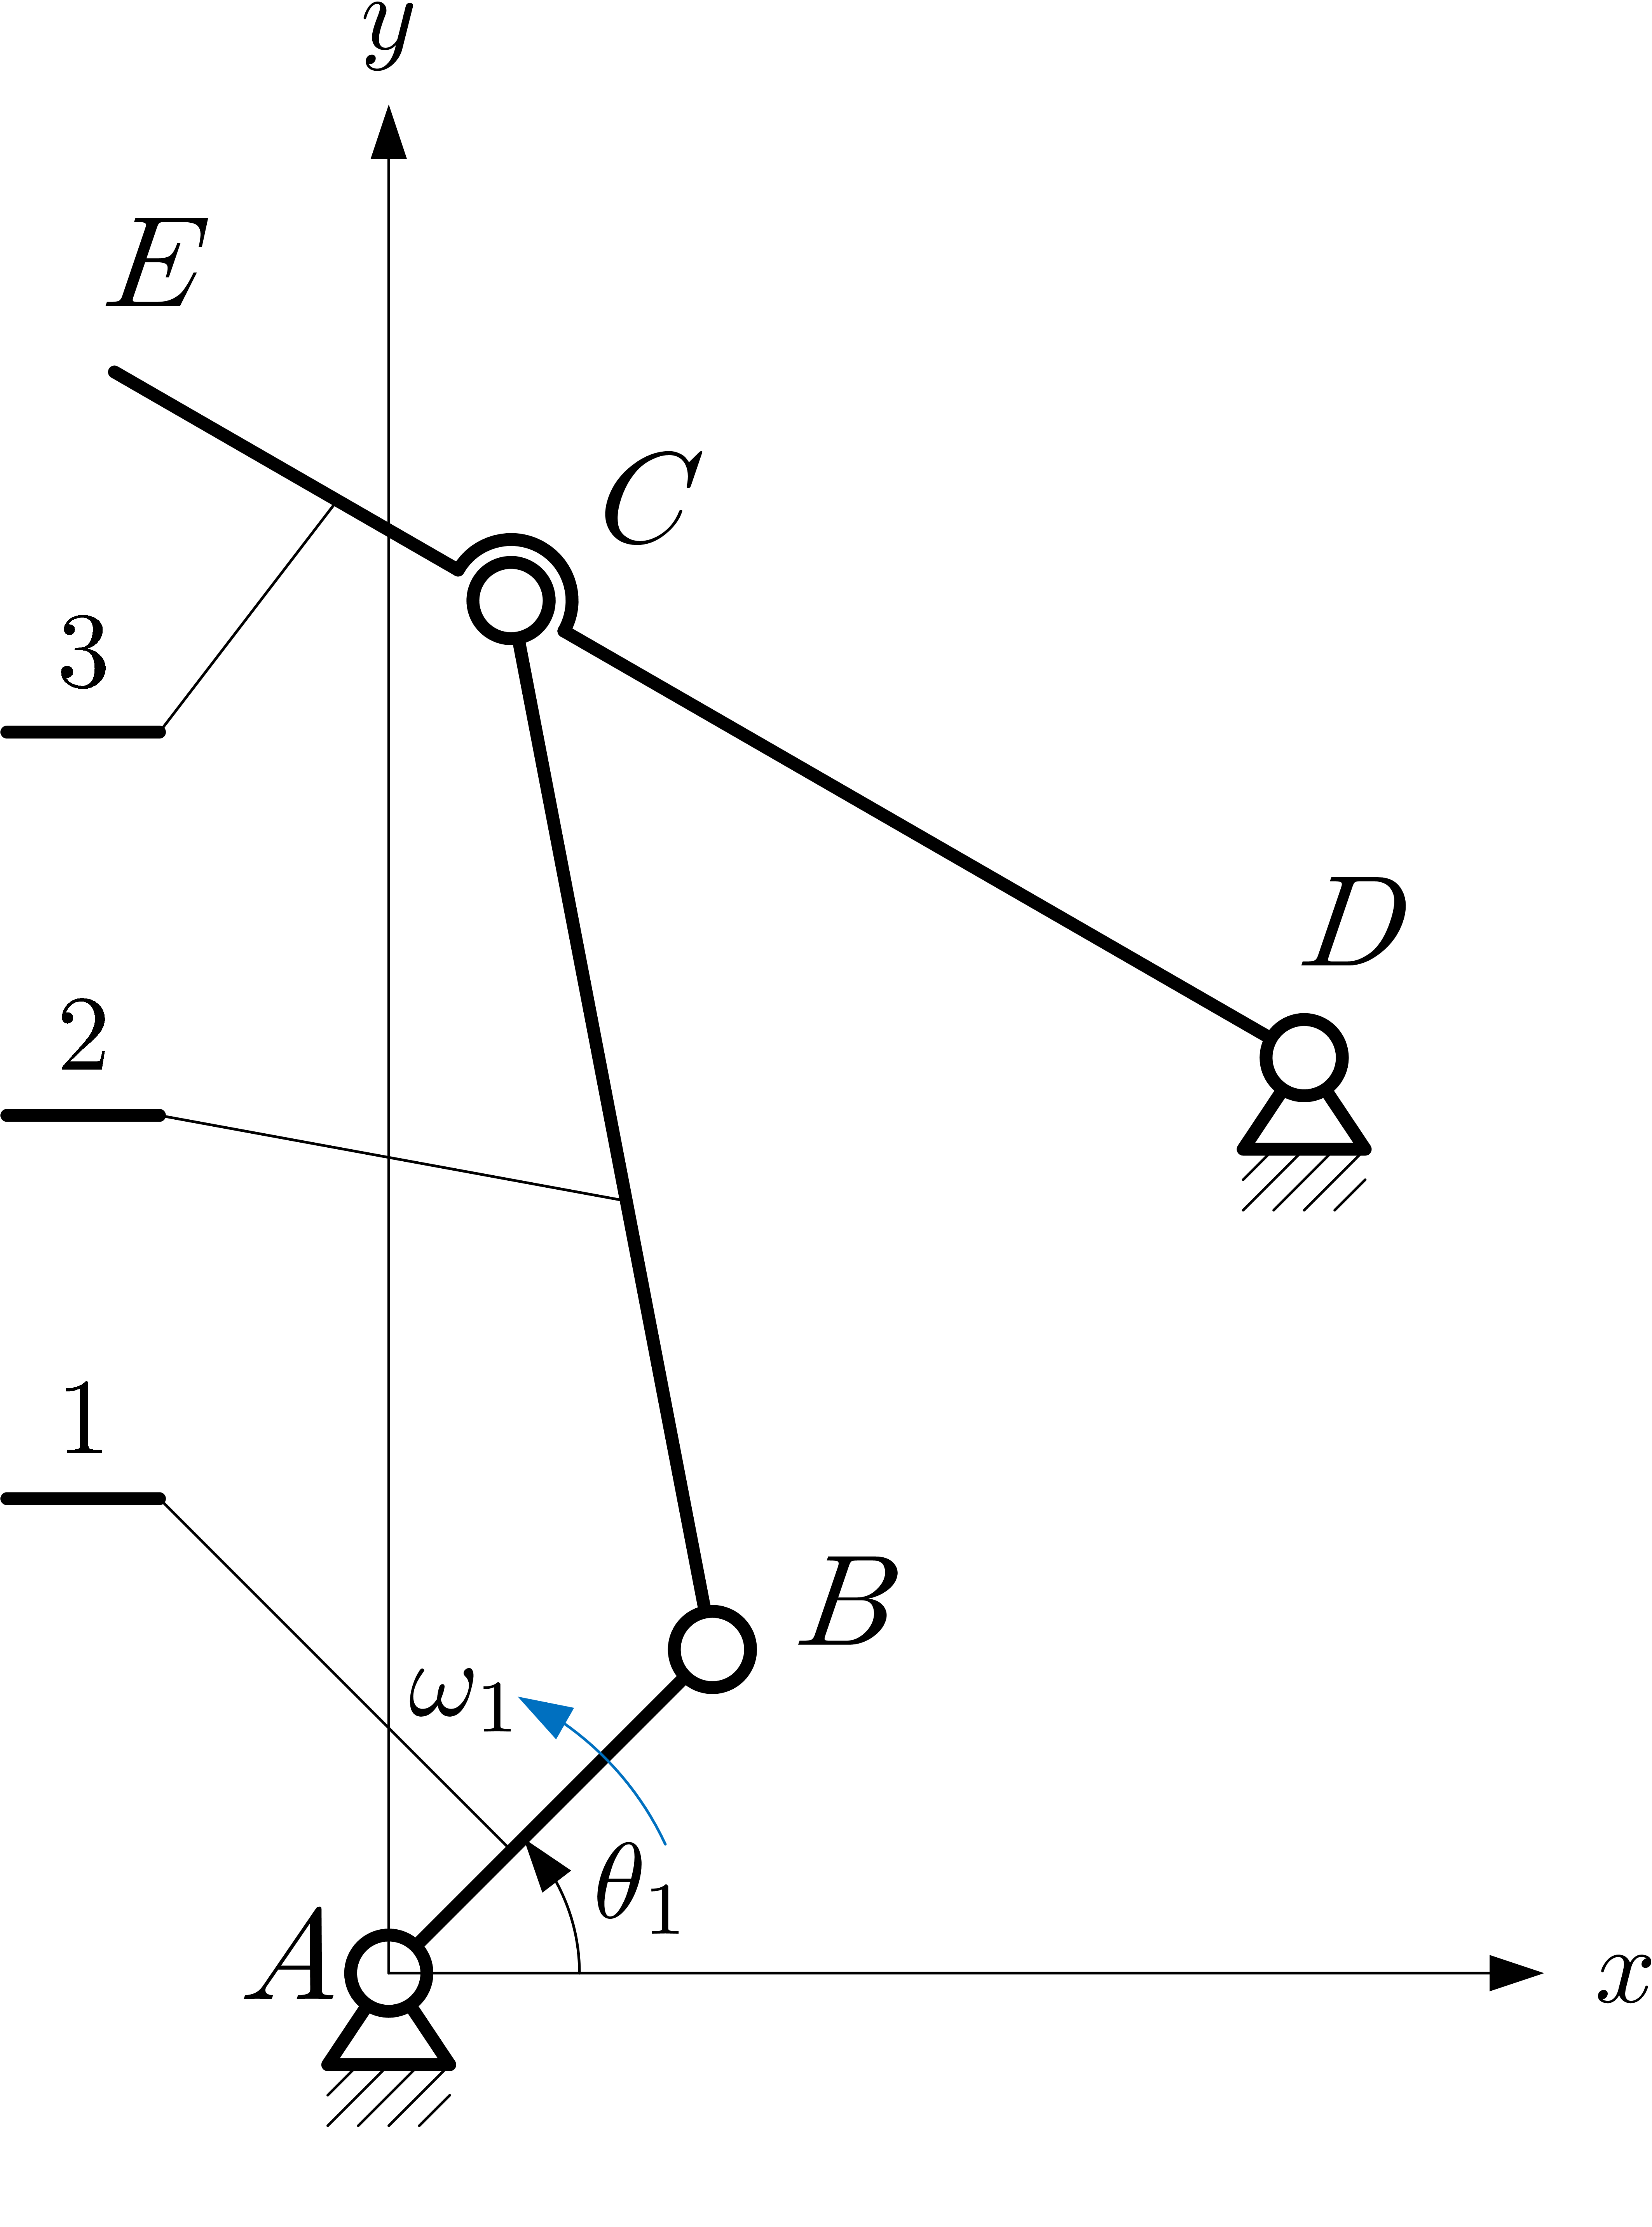
\includegraphics[width=50mm]{images/R-RRR.png}
				\end{figure}
			\end{minipage}
		\end{table}
	\end{block}
\end{frame}
\begin{frame}
	\emph{Solution}\vskip2.5mm
	Using position analysis / MATLAB,\vskip1.25mm
	$\vb{r}{B}=0.1061\ih+0.1061\jh$ $(m)$\\
	$\vb{r}{C}=0.0401\ih+0.4498\jh$ $(m)$\\
	$\vb{r}{E}=-0.0899\ih+0.5247\jh$ $(m)$\vskip1.25mm
	$\vb{r}{CD}=-0.2599\ih+0.1498\jh$ $(m)$\\ $\vb{r}{ED}=-0.3899\ih+0.2247\jh$ $(m)$\\ $\vb{r}{CB}=-0.066\ih+0.3437\jh$ $(m)$
\end{frame}
\begin{frame}
\begin{itemize}
	\item Find $\vb{v}{B}$\vskip1.25mm
	$\vb{v}{B} = \vb{\omega}{1}\times\vb{r}{B} = -0.6664\ih + 0.6664\jh$ $(m/s)$\vskip2.5mm
	
	\item Find $\vb{\omega}{2}$, $\vb{\omega}{3}$\vskip1.25mm
	$\vb{v}{C} = \vb{v}{B} + \vb{v}{CB} \Leftrightarrow\vb{\omega}{3}\times \vb{r}{CD}= \vb{v}{B} + \vb{\omega}{2}\times \vb{r}{CB}$\vskip2.5mm
	%$\omega_{3z}\kh\times(-0.2599\ih+0.1498\jh) = (-0.6664\ih + 0.6664\jh)$\\\hskip50mm $+\omega_{2z}\kh\times(-0.066\ih+0.3437\jh)$\vskip2.5mm
	Projecting onto $x,y$-axes, we obtain the solution:\vskip1.25mm
	$\Rightarrow\begin{cases}
	\omega_{3z} = -3.4364\text{ } (rad/s)\\ \omega_{2z}=-3.4364\text{ } (rad/s)
	\end{cases}$\\$\Rightarrow\begin{cases}
	\vb{\omega}{3} = -3.4364\kh\text{ }(rad/s)\\ \vb{\omega}{2}=-3.4364\kh\text{ }(rad/s)
	\end{cases}$\vskip2.5mm
	
	\item Find $\vb{v}{C}$, $\vb{v}{E}$\vskip1.25mm
	$\vb{v}{C}=\vb{\omega}{3}\times \vb{r}{CD}=0.5147\ih+0.8932\jh$ $(m/s)$, $\vb{v}{E}=\vb{\omega}{3}\times \vb{r}{ED}=0.7721\ih+1.3398\jh$ $(m/s)$
\end{itemize}
\end{frame}
	

\begin{frame}
		\begin{itemize}
			\item Find $\vb{a}{B}$, $\vb{a}{CB}^{\bm n}$, $\vb{a}{CD}^{\bm n}$\vskip1.25mm
			$\vb{a}{B} = \vb{\alpha}{1}\times \vb{r}{B} - \vb{\omega}{1}^2\vb{r}{B}=-4.1873\ih -4.1873\jh \text{ $(m/s^2)$}$\\
			$\vb{a}{CB}^{\bm n}=- \vb{\omega}{3}^2\vb{r}{CB}=0.7793\ih-4.0589\jh\text{ }(m/s^2)$\\
			$\vb{a}{CD}^{\bm n}=- \vb{\omega}{3}^2\vb{r}{CD}=3.0695\ih-1.7688\jh\text{ }(m/s^2)$\vskip2.5mm
			
			\item Find $\vb{\alpha}{2} = \alpha_{2z}\kh$, $\vb{\alpha}{3} = \alpha_{3z}\kh$\vskip1.25mm
			$\vb{a}{C} = \vb{a}{B} + \vb{a}{CB}\Leftrightarrow \vb{a}{CD}^{\bm t} + \vb{a}{CD}^{\bm n}= \vb{a}{B} + \vb{\alpha}{2}\times \vb{r}{CB} + \vb{a}{CB}^{\bm n}$\vskip2.5mm
%			$\alpha_{3z}\kh\times(-0.2599\ih+0.1498\jh) =-6.4774\ih-6.4774\jh+ \alpha_{2z}\kh\times(-0.066\ih+0.3437\jh)$\vskip2.5mm
			Projecting onto $x,y$-axes, we obtain the solution:\vskip1.25mm
			$\Rightarrow\begin{cases}
			\alpha_{3z} = -8.9788\text{ }(rad/s^2)\\\alpha_{2z}=22.6402\text{ }(rad/s^2)
			\end{cases}\Rightarrow\begin{cases}
			\vb{\alpha}{3} = -8.9788\kh\text{ }(rad/s^2)\\\vb{\alpha}{2}=22.6402\kh\text{ }(rad/s^2)
			\end{cases}$\vskip2.5mm
			\item Find $\vb{a}{C}$, $\vb{a}{E}$\vskip1.25mm
			$\vb{a}{C}=\vb{\alpha}{3}\times \vb{r}{CD}-\vb{\omega}{3}^2 \vb{r}{CD}=-0.3218\ih-7.6537\jh\text{ }(m/s^2)$\\ $\vb{a}{E}=\vb{\alpha}{3}\times \vb{r}{ED}-\vb{\omega}{3}^2 \vb{r}{ED}=-0.4827\ih-11.4805\jh\text{ }(m/s^2)$
		\end{itemize}
\end{frame}
\begin{frame}{MATLAB R2019a code}
\lstinputlisting[style=Matlab-editor, basicstyle=\mlttfamily]{codes/f-l_v.m}
\end{frame}
\begin{frame}{MATLAB R2019a code}
\lstinputlisting[style=Matlab-editor, basicstyle=\mlttfamily]{codes/f-l_v_2.m}
\end{frame}
\begin{frame}{MATLAB R2019a code}
\lstinputlisting[style=Matlab-editor, basicstyle=\mlttfamily]{codes/f-l_a.m}
\end{frame}
\begin{frame}{MATLAB R2019a code}
\lstinputlisting[style=Matlab-editor, basicstyle=\mlttfamily]{codes/f-l_a_2.m}
\end{frame}
\begin{frame}{Derivative Method}
	Let $\theta_1=\theta(t)$ be a function of time $t$. We perform position analysis with MATLAB to find $\vb{r}{B}(\theta(t))$, $\vb{r}{C}(\theta(t))$ and $\vb{r}{E}(\theta(t))$. Obtain the angle $\theta_2(\theta(t))$ of link 2 and $\theta_3(\theta(t))$ of link 3 using the results above.\vskip2.5mm
	Then, find velocities and accelerations by taking first and second derivative of $\vb{r}{B}$, $\vb{r}{C}$, $\vb{r}{E}$, $\theta_2$, $\theta_3$ respectively:
	\[\begin{cases}
	\displaystyle \vb{v}{B}(\theta(t))=\xvec[.]{\bm{r}}_{\bm{B}}\\\displaystyle \vb{v}{C}(\theta(t))=\xvec[.]{\bm{r}}_{\bm{C}}\\\displaystyle \vb{a}{E}(\theta(t))=\xvec[.]{\bm{r}}_{\bm{E}}\\\displaystyle \vb{\omega}{2}(\theta(t))=\dot{\theta_2}\kh\\\displaystyle \vb{\omega}{3}(\theta(t))=\dot{\theta_3}\kh
	\end{cases}, \begin{cases}
	\displaystyle \vb{a}{B}(\theta(t))=\xvec[:]{\bm{r}}_{\bm{C}}\\\displaystyle \vb{a}{C}(\theta(t))=\xvec[:]{\bm{r}}_{\bm{C}}\\\displaystyle \vb{a}{E}(\theta(t))=\xvec[.]{\bm{r}}_{\bm{E}}\\\displaystyle \vb{\alpha}{2}(\theta(t))=\ddot{\theta_2}\kh\\\displaystyle \vb{\alpha}{3}(\theta(t))=\ddot{\theta_3}\kh
	\end{cases}\]
	Let $\theta(t)=45^\circ$, we obtain the final results.
\end{frame}
\begin{frame}{MATLAB R2019a code}
\lstinputlisting[style=Matlab-editor, basicstyle=\mlttfamily]{codes/f-l_p_d.m}
\end{frame}
\begin{frame}{MATLAB R2019a code}
\lstinputlisting[style=Matlab-editor, basicstyle=\mlttfamily]{codes/f-l_p_d_2.m}
\end{frame}
\begin{frame}{MATLAB R2019a code}
\lstinputlisting[style=Matlab-editor, basicstyle=\mlttfamily]{codes/f-l_v_a_d.m}
\end{frame}
%\begin{frame}{MATLAB R2019a code}
%\lstinputlisting[style=Matlab-editor, basicstyle=\mlttfamily]{codes/f-l_a_d.m}
%\end{frame}
\begin{frame}{Independent Contour Method}
	Using the solution above,\vskip1.25mm
	$\vb{r}{B}=0.1061\ih+0.1061\jh$ $(m)$\\
	$\vb{r}{C}=0.0401\ih+0.4498\jh$ $(m)$\\
	$\vb{r}{E}=-0.0899\ih+0.5247\jh$ $(m)$
	\vskip1.25mm
	$\vb{r}{ED}=-0.3899\ih + 0.2247\jh$ $(m)$\\
	$\vb{r}{DC}= 0.2599\ih - 0.1498\jh$ $(m)$\\
	$\vb{r}{CB}= -0.066\ih + 0.3437\jh$ $(m)$
	\vskip1.25mm
	$\vb{a}{B}=0.183\ih-0.683\jh$ $(m/s^2)$
\end{frame}

\begin{frame}
Applying velocity formulas to find $\vb{\omega}{12} = \omega_{12z}\kh$, $\vb{\omega}{23} = \omega_{23z}\kh$,
$\vb{\omega}{30} = \omega_{30z}\kh$:\vskip1.25mm
$\begin{cases}
\vb{\omega}{01} + \vb{\omega}{12} + \vb{\omega}{23} + \vb{\omega}{30} = \vb{0}{}\\
\vb{r}{B}\times\vb{\omega}{12} + \vb{r}{C}\times\vb{\omega}{23} + \vb{r}{D}\times\vb{\omega}{30} = \vb{0}{}
\end{cases}$\vskip2.5mm
%\\$\Rightarrow\begin{cases}
%1\kh+\omega_{12z}\kh + \omega_{23z}\kh + \omega_{30z}\kh=\vb{0}{}\\
%(0.1061\ih+0.1061\jh)\times\omega_{12z}\kh+(0.0401\ih+0.4498\jh)\times\omega_{23z}\kh\\
%\hskip50mm+(0.3\ih+0.3\jh)\times\omega_{30z}\kh=\vb{0}{}
%\end{cases}$\vskip2.5mm
	Solving the system of equations by projecting onto $x,y$-axes, we obtain:\vskip1.25mm
	$\vb{\omega}{12} = -9.7196\kh\text{ }(rad/s)$, 
	$\vb{\omega}{23} = \vb{0}{}\text{ }(rad/s)$, 
	$\vb{\omega}{30} = 3.4364\kh\text{ }(rad/s)$\vskip2.5mm
	The results is consistent with the 2 previous methods.
\end{frame}

\begin{frame}
Again, using acceleration formulas to find $\vb{\alpha}{12} = \alpha_{12z}\kh$, 
$\vb{\alpha}{23} = \alpha_{23z}\kh$, 
$\vb{\alpha}{30} = \alpha_{30z}\kh$:\vskip1.25mm
$\begin{cases}
\vb{\alpha}{01} + \vb{\alpha}{12} + \vb{\alpha}{23} + \vb{\alpha}{30} = \vb{0}{}\\
\vb{r}{B}\times\vb{\alpha}{12} + \vb{r}{C}\times\vb{\alpha}{23} + \vb{r}{D}\times\vb{\alpha}{30} - \vb{\omega}{1}^2\vb{r}{B} - \vb{\omega}{2}^2\vb{r}{CB} - \vb{\omega}{3}^2\vb{r}{DC} = \vb{0}{}
\end{cases}$\vskip2.5mm%\\$\Rightarrow\begin{cases}
%-1\kh+\alpha_{12z}\kh + \alpha_{23z}\kh+\alpha_{30z}\kh=\vb{0}{}\\
%(0.1061\ih+0.1061\jh)\times\alpha_{12z}\kh+(0.0401\ih+0.4498\jh)\times\alpha_{23z}\kh\\\hskip30mm+(0.3\ih+0.3\jh)\times\vb{\alpha}{30}\kh-6.4774\ih-6.4774\jh=\vb{0}{}
%\end{cases}$\vskip2.5mm
Solving the system of equations by projecting onto $x,y$-axes, we obtain:\vskip1.25mm $\vb{\alpha}{12} = -8.9788\kh\text{ }(rad/s^2)$\\ $\vb{\alpha}{23} = 31.619\kh\text{ }(rad/s^2)$\\
$\vb{\alpha}{30} = -22.6402\kh\text{ }(rad/s^2)$\vskip2.5mm
The results is consistent with the 2 previous methods.
\end{frame}
\begin{frame}{MATLAB R2019a code}
\lstinputlisting[style=Matlab-editor, basicstyle=\mlttfamily]{codes/f-l_v_i.m}
\end{frame}
\begin{frame}{MATLAB R2019a code}
\lstinputlisting[style=Matlab-editor, basicstyle=\mlttfamily]{codes/f-l_v_i_2.m}
\end{frame}
\begin{frame}{MATLAB R2019a code}
\lstinputlisting[style=Matlab-editor, basicstyle=\mlttfamily]{codes/f-l_a_i.m}
\end{frame}
\begin{frame}{MATLAB R2019a code}
\lstinputlisting[style=Matlab-editor, basicstyle=\mlttfamily]{codes/f-l_a_i_2.m}
\end{frame}
\begin{frame}{Velocity - Acceleration plotting}
\lstinputlisting[style=Matlab-editor, basicstyle=\mlttfamily]{codes/f-l_v_a_plotting.m}
\end{frame}
\begin{frame}{Output figures}
\begin{table}
	\begin{minipage}{0.5\linewidth}
		\begin{figure}
			\centering
			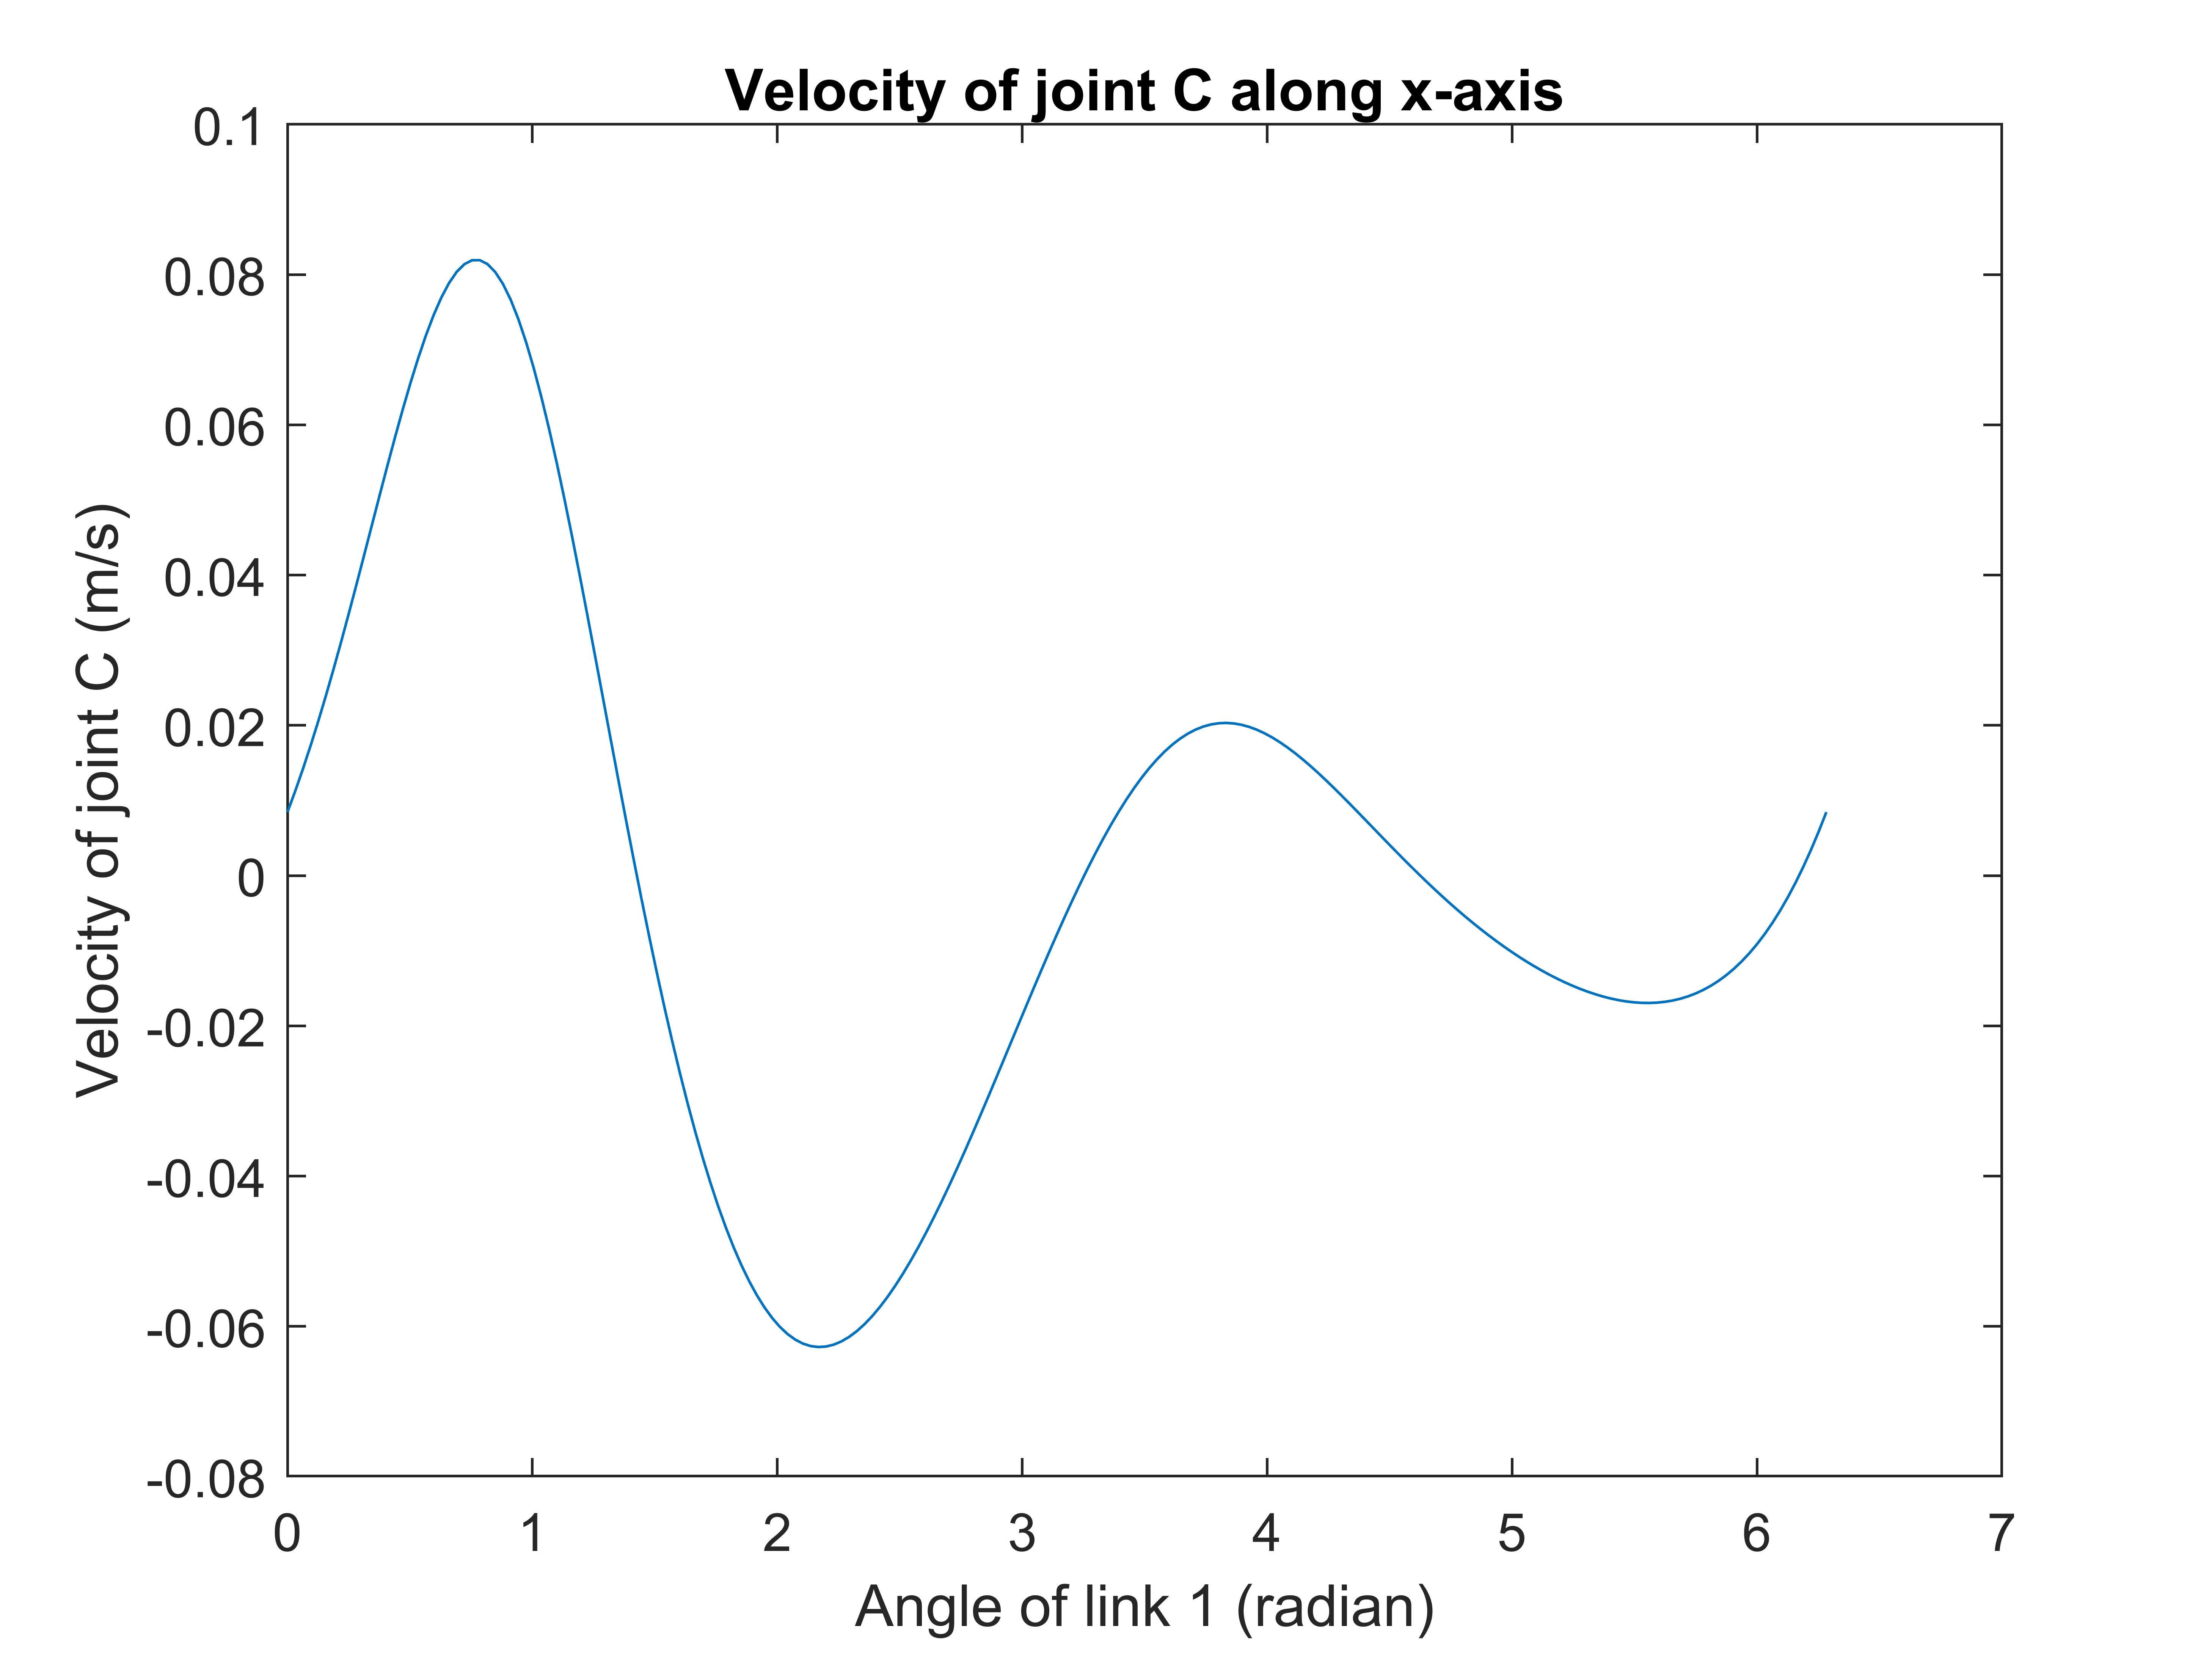
\includegraphics[width=60mm]{images/v_RRRR.png}
		\end{figure}
	\end{minipage}\hfill
	\begin{minipage}{0.5\linewidth}
		\begin{figure}
			\centering
			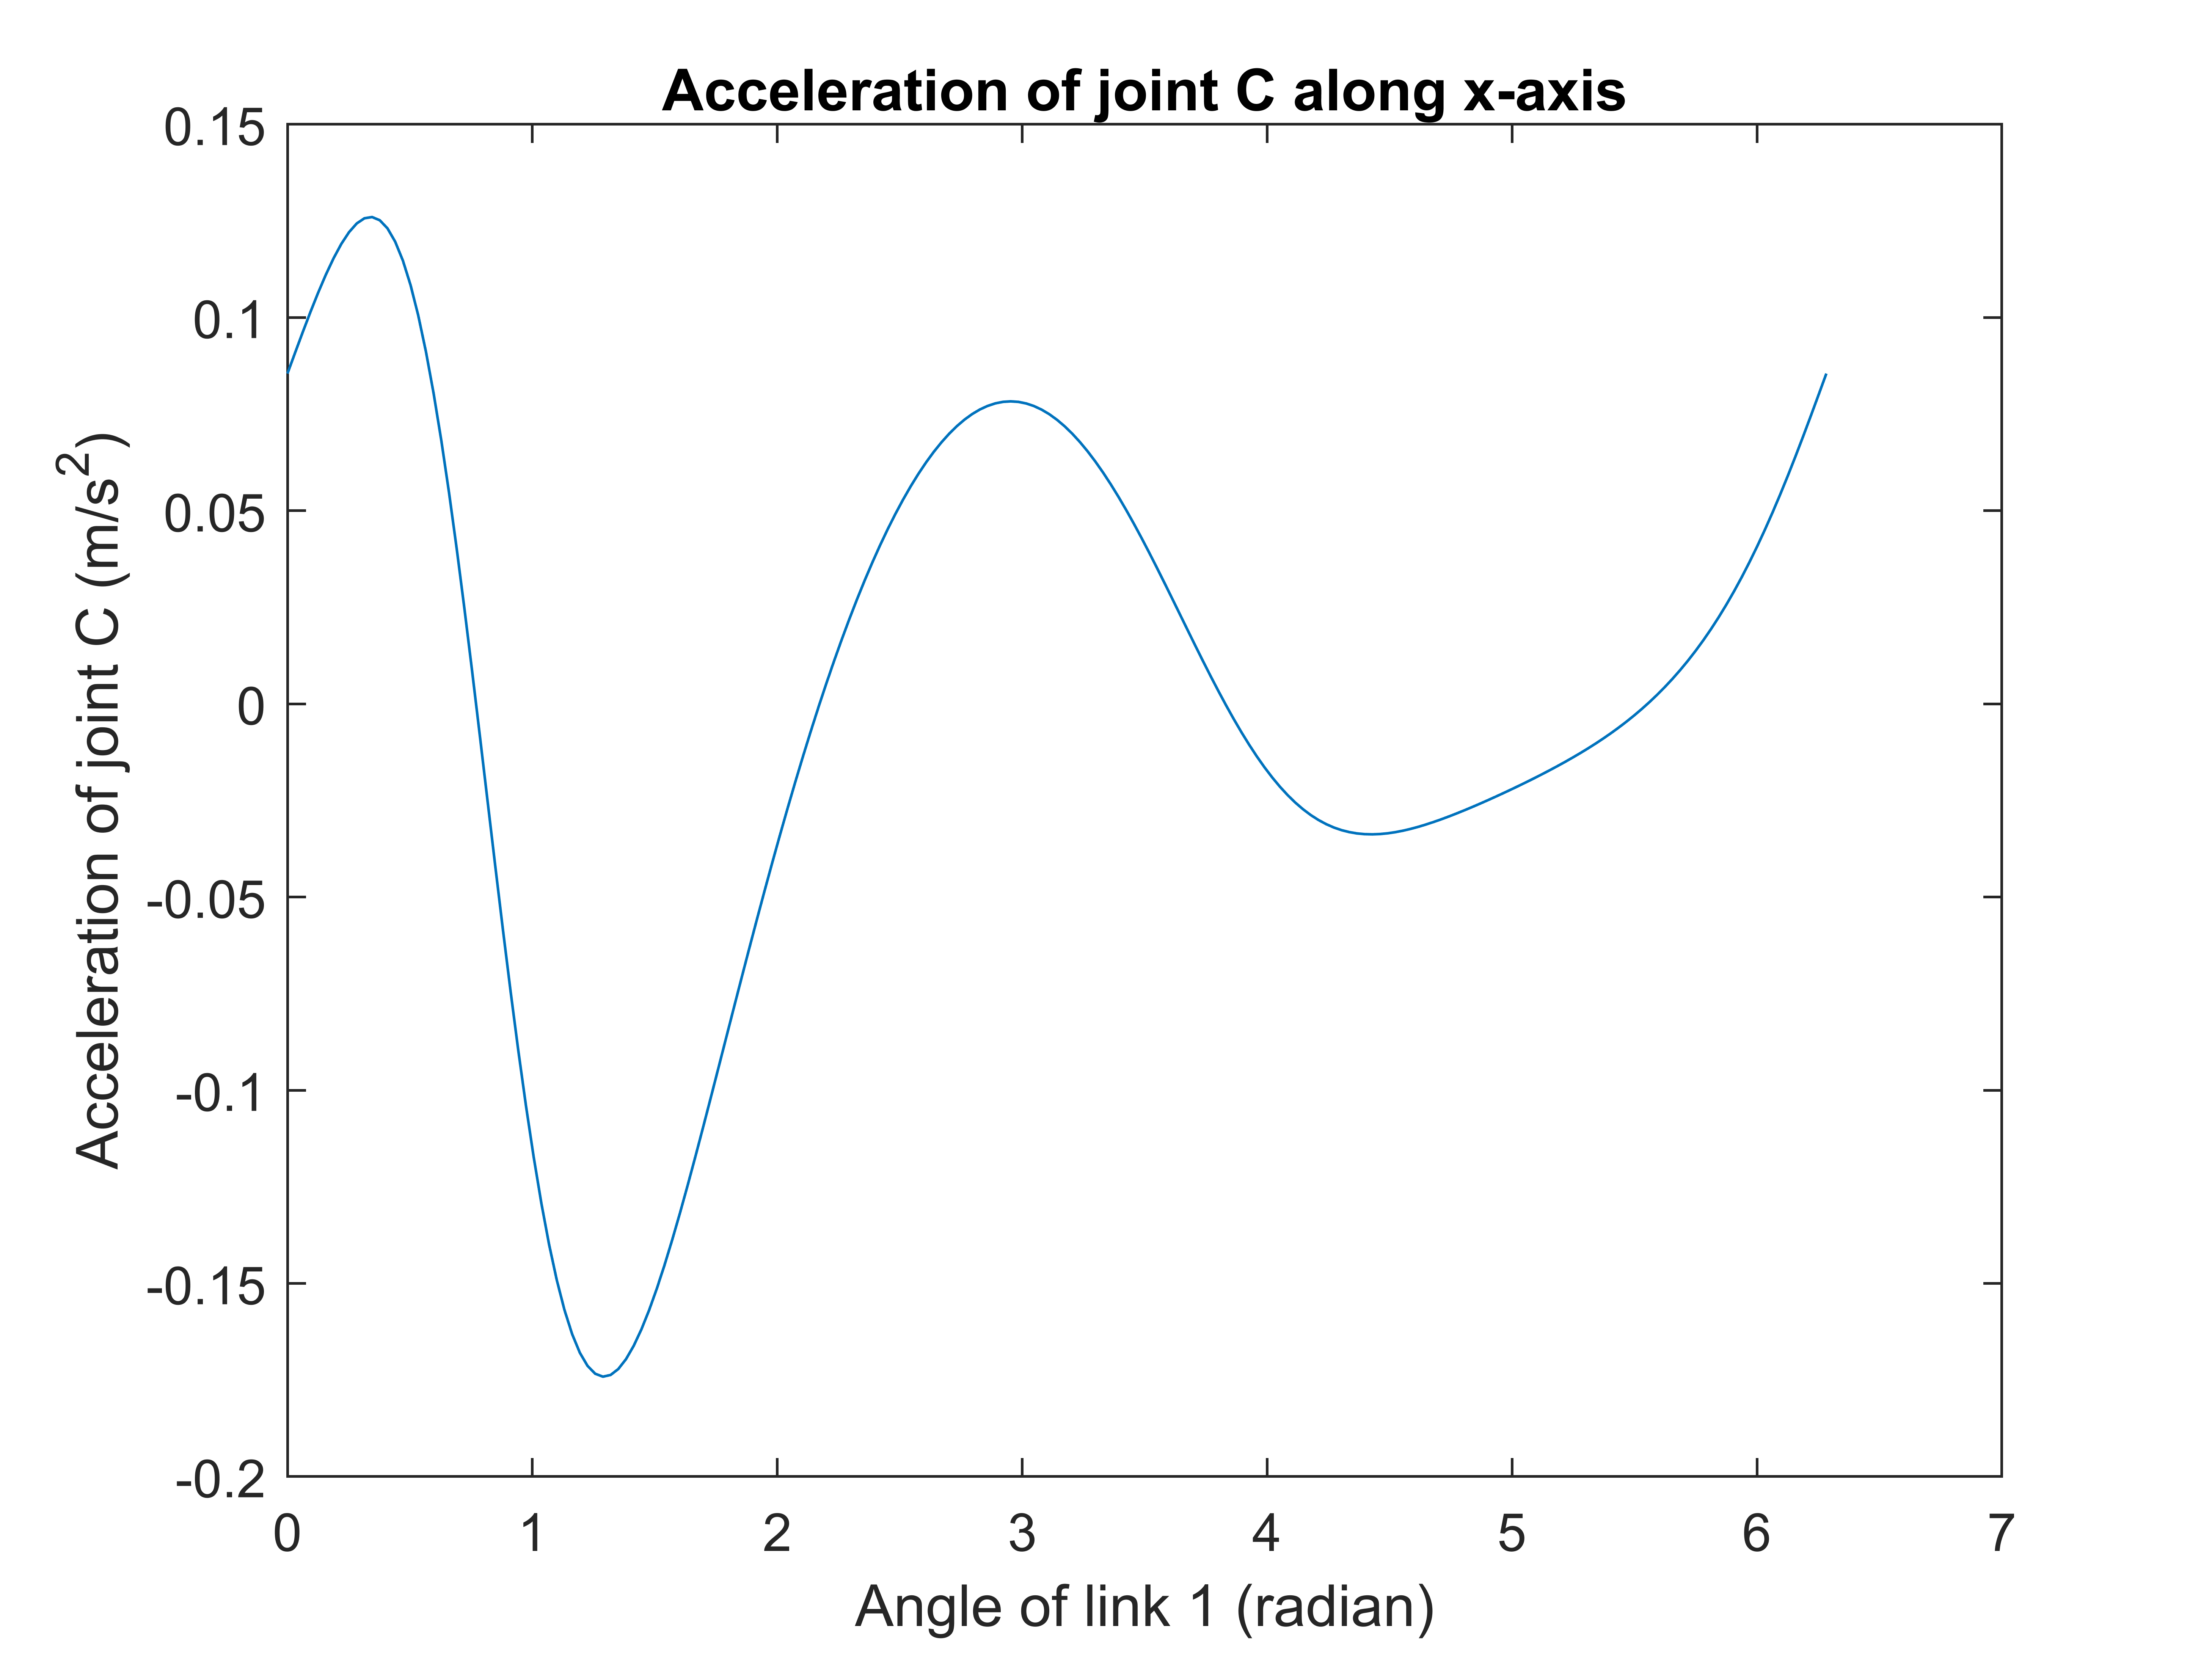
\includegraphics[width=60mm]{images/a_RRRR.png}
		\end{figure}
	\end{minipage}
\end{table}
\end{frame}